\chapter{État de l'art}

En effectuant nos recherches sur le sujet nous avons trouvé beaucoup d'informations sur les abeilles et le travail des apiculteurs en général, ainsi que des systèmes "maison" développés par des particuliers pour surveiller un peu mieux leurs ruches. Cependant nous avons également découvert l'existence de quatre projets similaires au notre: trois projets en cours ayant une approche OpenSource et un projet commercial déjà développé. Ce dernier appartient à la société anglaise Arnia. Ce système est décrit \cite{arnia} comme permettant à l'utilisateur d'avoir des informations sur une ou plusieurs ruches telles que la température, l'humidité et l'intensité acoustique dans la ruche ainsi que la température du couvain. Les apiculteurs peuvent ensuite visualiser ces informations sur une partie sécurisée du site internet d'arnia. Ils peuvent également comparer les informations et évolution d'une ou plusieurs ruches, comme on peut le voir sur la figure \ref{fig:arnia1}.

\begin{figure}[h]
\centering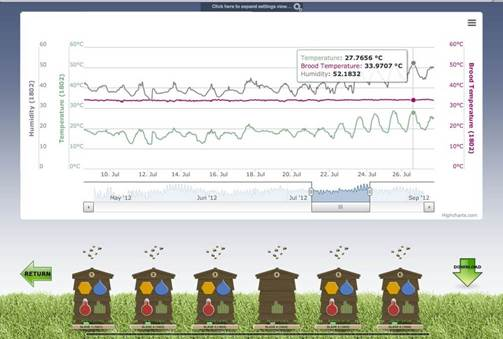
\includegraphics{arnia1.jpg}
\caption{\label{fig:arnia1} Interface du système d'arnia: comparaison des données d'une ruche}
\end{figure}

L'un des projets OpenSource est développé par Ken Meyer sur le site hackaday \cite{hackaday} et consiste à mesurer la température, l'humidité et le poids d'une ruche. Ce projet est encore en développement et plusieurs prototypes ont déjà été testés.

Il existe également un autre projet OpenSource sur le sujet. Il s'agit de Bzzz \cite{projetBzzz}, développé par le Fablab de Lannion. Ce système propose une supervision de la température intérieure, de la luminosité extérieure et la masse d'une seule ruche via un envoi de données périodique par SMS et par visualisation des données sur un portail en ligne. L'utilisateur pourra également configurer des alertes via le portail.

Enfin le dernier système existant que nous avons trouvé a été développé conjointement par le Fablab de Barcelone et Open Tech Collaborative, Denver, USA \cite{OpenBeehives}. Ce projet OpenSource, appelé Open Source BeeHive, ne s'adapte pas aux ruches classiques mais propose une architecture simple qui permet de construire sa propre ruche entièrement, comme on peut le voir sur les figures \ref{fig:OSBH2} et \ref{fig:OSBH}.

\begin{figure}[h]
\centering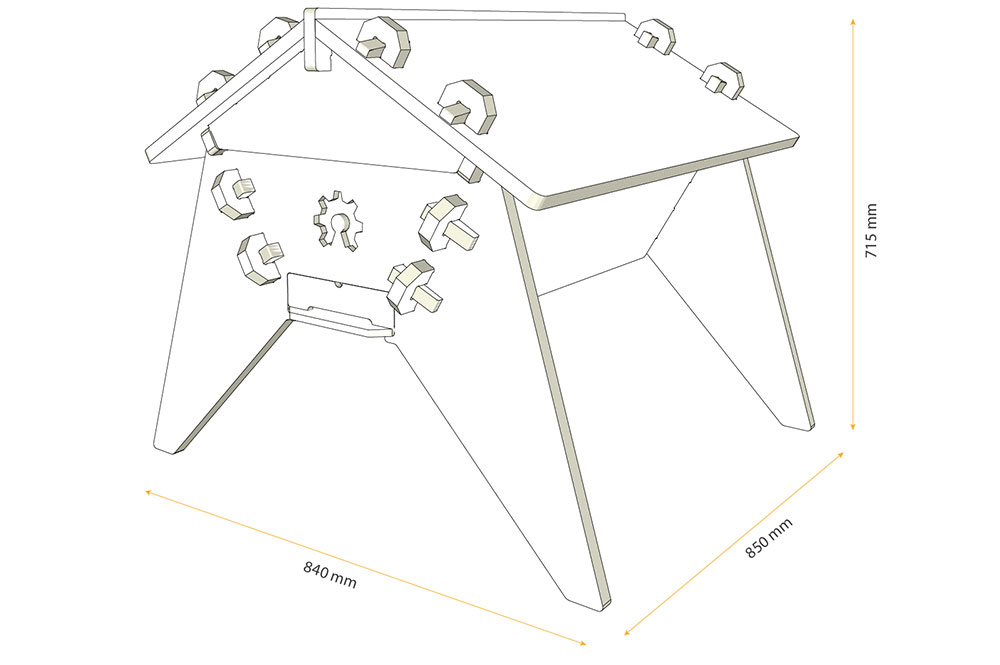
\includegraphics[scale=0.3]{OSBH.jpg}
\caption{\label{fig:OSBH} Modèle de ruche Open Source Beehive}
\end{figure}

\begin{figure}[h]
\centering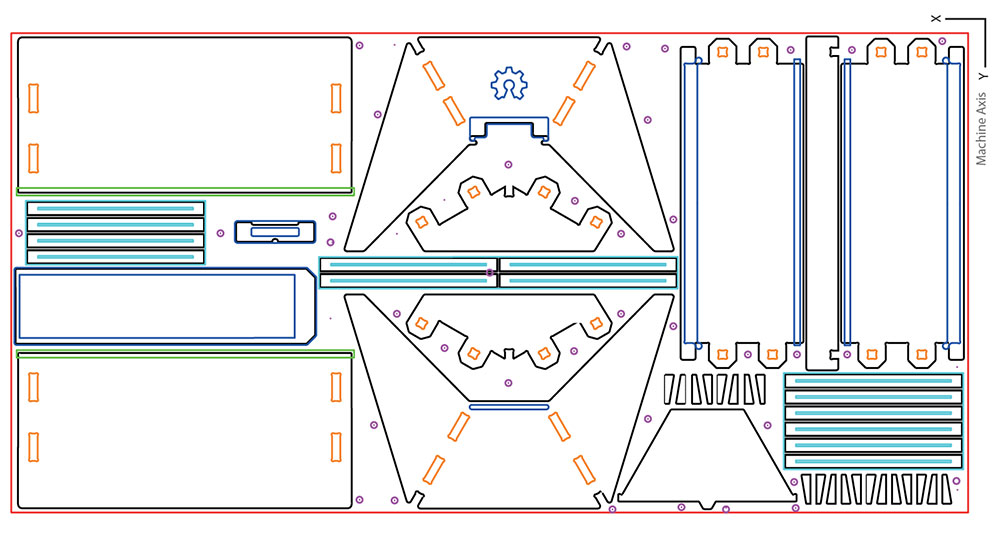
\includegraphics[scale=0.3]{OSBH2.jpg}
\caption{\label{fig:OSBH2} Plan de la ruche Open Source Beehive}
\end{figure}

Ensuite un kit de capteurs à installer permet de mesurer la température, l'humidité, l'intensité acoustique et le nombre d'abeilles via un capteur infrarouge. Les données seront ensuite visibles de tous sur la plateforme Smart Citizen.

Nous n'avons pas détaillé ici tous les projets que nous avons trouvés du fait de leur grand nombre. Cependant nous nous sommes intéressés à ceux qui présentaient un intérêt pour le système que nous voulons développer. 

Concernant le traitement sonore, le site internet Beesource comporte une description complète du système Apidictor \cite{apidictor}. Ce système permet de filtrer le son émit par une ruche pour prévoir un essaimage. Un schéma du montage électrique ainsi qu'un texte expliquant quelles fréquences sont surveillées et quelles méthodes ont été utilisées pour vérifier le bon fonctionnement de ce système sont également présents. Nous ne réutiliserons pas le montage proposé, car le traitement du signal sonore se fera de manière informatisée, en revanche le travail effectué pour savoir quelles fréquences sont à surveiller nous sera utile.

\section{Choix des capteurs}

Après avoir réalisé l'état de l'art pour notre système de surveillance d'une ruche, nous nous sommes ensuite intéressés aux capteurs que nous allons employer.

Capteur de température

Nous avons choisis un capteur de température identique pour recueillir la température interne et externe de la ruche.
Il s'agit d'une thermistance NTC boitier Goutte Radial 1000 ohms sortie fil de cuivre émaillé 1 pc(s). Ce dernier possède une gamme de mesure comprise entre -40°C et 100°C ce qui correspond bien aux exigences discutées avec le client (Voir tableau des exigences).

Capteur d'humidité

On a choisit d'inclure ce capteur dans notre système compte tenu des résultats de l'Etat de l'art. Néanmoins, après discussion avec le client, cette option n'est pas primordiale pour un apiculteur.

Capteur de pression
Les capteurs de pression vont nous permettre de récupérer le poids de ruche et surtout celui des hausses pour avertir l'apiculteur de la quantité de miel produite. Pour se faire, le projet Bzzz développé par le Fablab de Lannion a prévu d'utiliser deux sachets de Pompote remplis d'eau sucrée pour éviter les variations de pression atmosphérique, le gel et l'évaporation. Cependant, après avoir pris conscience de l'importance de la localisation de la grappe, nous avons pensé installer deux capteurs de pression par cadre (au niveau de chaque extrémité) soit 20 au total mais cette solution s'est avérée être difficile à mettre en place à cause de la surface sur laquelle repose les cadres (simple lamelle en métal). Après discussion avec le client, nous avons finalement opté pour la confection d'un cadre en bois aux même dimensions de la ruche dans lequel se trouverons les capteurs de pression. L'utilisateur décidera de l'endroit où le placer en fonction des données qu'il veut récupérer.    

Tilt sensor 

Ce capteur

Microphone

 
  